\subsection{Fönster}

\subsubsection{Solens position och intensitet}
\begin{frame}{Solens position}
  \begin{center}
  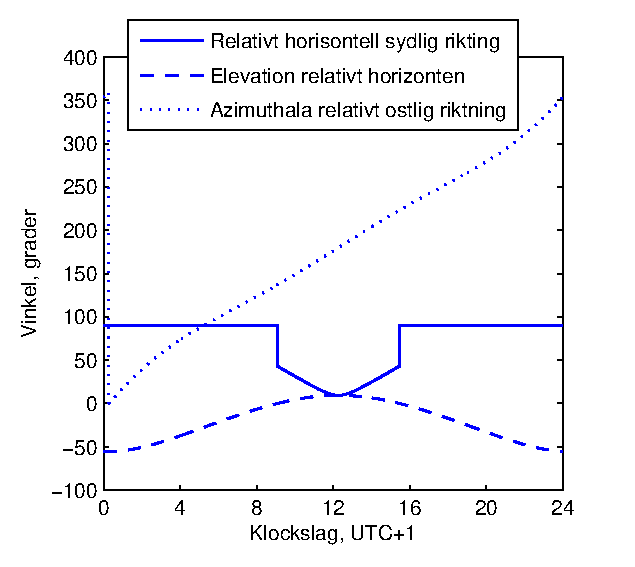
\includegraphics[scale=0.8]{images/sunposition1231.eps}
  \end{center}
\end{frame}

\subsubsection{Direkt strålning, konduktion, konvektion och IR}
\begin{frame}{Flöden genom fönster}
  \begin{align*}
    g\left( \theta \right) & = g_0 \cdot p\left( \theta \right)\\[10pt]
    p\left( \theta \right) & \propto \text{Antal rutor \& beläggningar}\\[10pt]
    Q_{\text{sol}} \,\,\,\, & = g\left( \theta \right) \cdot I_0 \cos{\left( \theta \right)}\\[10pt]
    Q_{\text{kond}} & = \frac{1}{\frac{1}{U}+\frac{1}{h}} \left( T_{inne} - T_{ute}\right)\\[10pt]
    Q_{\text{långvåg}} & = 0,75 \cdot \sigma \left( T_{inne}^4 - T_{ute}^4\right)
  \end{align*}
\end{frame}

% Se Karlsson, J. och Roos, A. (2000) för g-värden
% Förklaring av hur vi räknat med S-B:s lag
% Diffus strålning och omedelbar reflektion borträknat

\subsubsection{Totalt genom fönster}
\begin{frame}{Flöden genom fönster}
  Bild på alla flöden som ges av föregående slide
\end{frame}
